%% LaTeX-Beamer template for KIT design
%% by Erik Burger, Christian Hammer
%% title picture by Klaus Krogmann
%%
%% version 2.0
%%
%% mostly compatible to KIT corporate design v2.0
%% http://intranet.kit.edu/gestaltungsrichtlinien.php
%%
%% Problems, bugs and comments to
%% burger@kit.edu

\documentclass[18pt]{beamer}
\usetheme{kit}

%% TITLE PICTURE

% if a custom picture is to be used on the title page, copy it into the 'logos'
% directory, in the line below, replace 'mypicture' with the 
% filename (without extension) and uncomment the following line
% (picture proportions: 63 : 20, *.eps format if you use latex+dvips+ps2pdf,
% *.jpg/*.png/*.pdf if you use pdflatex)

%\titleimage{mypicture}

%% TITLE LOGO

% for a custom logo on the front page, copy your file into the 'logos'
% directory, insert the filename in the line below and uncomment it

%\titlelogo{mylogo}

% (*.eps format if you use latex+dvips+ps2pdf,
% *.jpg/*.png/*.pdf if you use pdflatex)

%% BIBTEX ICON/KEY

% if you want to see BibTeX keys in the references view instead of the symbol,
% uncomment the following line
% \usebibitemtemplate{\insertbiblabel}

% the presentation starts here

% change the following line to "ngerman" for German style date and logos
% change the following line to "english" for English style date and logos
\selectlanguage{ngerman}

\beamertemplatenavigationsymbolsempty

\usepackage{listings}
\definecolor{darkgray}{rgb}{0.95,0.95,0.95}
\definecolor{darkgreen}{rgb}{0.05,0.7,0.05}
\lstset{ language=Java,
	backgroundcolor=\color{darkgray}, 
	numbers=none, 
	keywordstyle=\color{black}\bfseries,
	tabsize=2,
	showspaces=false,               % show spaces adding particular underscores
	showstringspaces=false,         % underline spaces within strings
	showtabs=false, 
}



\title[Tutorium04]{Tutorium 04: Entwurfsmuster}
\subtitle{Softwaretechnik im SS 2011, Tutorium 4}
\author{Jürgen Walter}
\date{\today}

\institute{Chair for Software Design and Quality}

\begin{document}

%title page
\begin{frame}
\titlepage
\end{frame}

%table of contents
\frame{
\frametitle{Was machen wir heute?}
	\tableofcontents
}

\section{Altes Übungsblatt}

\subsection{Altes Übungsblatt}
\frame {
\frametitle{Altes Übungsblatt}
	\begin{block}{Aufgabe 1 - UML Zustandautomaten}
	\begin{itemize}
	\item Start- und Endzustand nicht vergessen!
	\item Bei Nebenläufigen Zustandsautomaten ist beim transformierten Automaten ein ,,guter'' Name A$\times$B für einen Zustand
	\end{itemize}
	\end{block}
}


\begin{frame}[fragile]
\frametitle{Altes Übungsblatt}
	\begin{block}{Aufgabe 2 - Überladen und Überschreiben}
	\begin{itemize}
	\item Super! Hat jeder verstanden.
	\end{itemize}
	\end{block}
	\pause
	\begin{block}{Aufgabe 3 - JMJRST erweitern} 
	\begin{itemize}
	\item ???
	\end{itemize}
	\end{block}
\end{frame}

\frame{
\frametitle{Altes Übungsblatt}
	\begin{block}{Bonusaufgabe - Kammerjäger}
	\begin{itemize}
	\item wer hat den Debugger benutzt?
	\item bla?
	\end{itemize}
	\end{block}
}

\subsection{Zum Aufwärmen ...}
\frame {
\frametitle{Wahr oder falsch?}
\begin{itemize}
	\color<2->[rgb]{1,0,0}
	\item Fassade und Adapter gehören zu den Bequemlichkeitsmustern.
	\color[rgb]{0,0,0}
	\pause
	\color<3->[rgb]{0,1,0}
	\item Das Entwurfsmuster „Abstrakte Fabrik“ konzentriert sich auf den schrittweisen Konstruktionsprozess komplexer Objekte. geändert werden.
	\color[rgb]{0,0,0}
	
	\pause
	\color<4->[rgb]{0,1,0}
	\item Eine Fabrikmethode kann eine Einschubmethode bei einer Schablonenmethode für Objekterzeugung sein.
	\color[rgb]{0,0,0}
	\pause
	\color<5->[rgb]{1,0,0}
	\item In Java muss eine Klasse, die eine Schnittstelle implementiert, alle in der Schnittstelle vorgegebenen Methoden implementieren
	\color[rgb]{0,0,0}
	\pause
	\color<6->[rgb]{1,0,0}
	\item In Java ist das Entwurfsmuster „Null-Objekt“ durch das Schüsselwort null realisiert.
	\color[rgb]{0,0,0}

\pause
	\color<7->[rgb]{0,1,0}
	\item Wenn eine Klasse eine abstrakte Methode besitzt, dann ist sie auch selbst abstrakt.
	\color[rgb]{0,0,0}

\pause
	\color<8->[rgb]{0,1,0}
	\item Zusicherungen (z.B. mit dem Schlüsselwort assert in Java) werden zur Laufzeit eines Programs ausgeführt.
	\color[rgb]{0,0,0}
\end{itemize}
}

\frame {
\frametitle {Klausuraufgaben zum Aufwärmen} 
	\begin{block} {Aufgabe 1 (1P)}
	Nennen Sie genau zwei Gründe, die laut Vorlesung für den Einsatz von Entwurfsmustern sprechen. \\
	\visible<2-> {
	\begin{itemize}
		\item verbessern die Kommunikation im Team
		\item erfassen wesentliche Konzepte und bringen sie in eine verständliche Form
		\item helfen Entwürfe zu verstehen
		\item dokumentieren Entwürfe kurz und knapp
		\item dokumentieren und fördern den Stand der Kunst
		\item helfen weniger erfahrenen Entwerfern
		\item vermeiden die Neuerfindung des Rades
		\item können Code-Qualität und Code-Struktur verbessern
		\item fördern gute Entwürfe und guten Code
	\end{itemize}
	}
	\end{block}
}

\frame {
\frametitle {Klausuraufgaben zum Aufwärmen} 
	\begin{block} {Aufgabe 2 (2P)}
	In der Konfigurationsverwaltung haben Sie zwei Alternativen kennengelernt, Änderungen an versionierten Dateien zu speichern. Nennen und beschreiben Sie die beiden Alternativen kurz. Nennen Sie für jede Alternative je einen Vorteil.\\
	\visible<2-> {
	\begin{itemize}
		\item Vorwärtsdeltas speichern eine Grundversion und die daran durchgeführten Änderungen
		\item Rückwärtsdeltas speichern die aktuelle Version und die Änderungen für frühere Versionen
		\item Vorteil Vorwärtsdelta: Schneller Zugriff auf frühere Versionen
		\item Vorteil Rückwärtsdelta: Schneller Zugriff auf aktuelle Versionen
	\end{itemize}
	}
	\end{block}
}

\frame {
\frametitle {Klausuraufgaben zum Aufwärmen} 
	\begin{block} {Aufgabe 3 (3P)}
In der Vorlesung wurden für den Vergleich zweier Objekte mehrere Stufen von Gleichheit definiert. Geben Sie die Definitionen für Gleichheit 0. und 1. Stufe an. \\
	\visible<2-> {
	\begin{itemize}
		\item Gleichheit 0. Stufe: Es handelt sich um dasselbe Objekt, die Objekte sind identisch.
		\visible<3-> {
		\item Gleichheit 1. Stufe: Es handelt sich entweder um dasselbe Objekt oder zwei verschiedene Objekte, die aber in allen Attributen/Assoziationen identische Werte besitzen (Gleichheit 0. Stufe oder paarweise Gleichheit 0. Stufe in allen Attributen)
		}
	\end{itemize}
	}
	\end{block} 
}

\section{Entwurfsmuster}

\frame{
\frametitle {Entwurfsmuster - Überblick}
	\begin{itemize}
		\item Entkopplungsmuster
		
		\begin{itemize}
			\item Adapter, Beobachter, Brücke, Iterator, Stellvertreter, Vermittler
		\end{itemize}
		
		\item Varianten-Muster
		\begin{itemize}
			\item Abstrakte Fabrik, Besucher, Fabrikmethode, Kompositum, Schablonenmethode, Strategie
		\end {itemize}
		\item Zustandshandhabungs-Muster
		\begin{itemize}
			\item Einzelstück, Fliegengewicht, Memento, Prototyp, Zustand
		\end{itemize}
		\item Steuerung-Muster
			\begin{itemize}
				\item Befehl, Master/worker
		\end{itemize}
		\item Virtuelle Maschinen
		\item Bequemlichkeitsmuster
			\begin{itemize}
				\item Bequemlichkeits-Klasse, Bequemlichkeits-Methode, Fassade, Null-Objekt
		\end{itemize}
	\end{itemize}


}

\frame {
\frametitle {Klausuraufgabe 2006} 
	\begin{block} {Aufgabe (5)}
Ein binärer arithmetischer Ausdruck enthält einen Operanden, einen Operator (+ - * /) und einen anderen Operanden. Die Operanden können entweder eine Zahl sein oder selbst wieder ein anderer binärer arithmetischer Ausdruck. Entwerfen Sie mit Hilfe eines Entwurfsmusters ein Klassendiagramm, um die Bestandteile eines binären arithmetischen Ausdrucks zu einer Baumstruktur zusammenzufügen und seine Bestands-Hierarchien zu repräsentieren. Nennen Sie das verwendete Entwurfsmuster. Hinweis: z.B. 2 + 3 und (2 + 3) + (4 * 6) sind beide gültige arithmetische Ausdrücke. (5 P)
	\end{block} 

Welches Entwurfsmuster sollte man hier verwenden?
\visible<2-> {
	Kompositum
}
}


\frame {
\frametitle {Kompositum Allgemeines} 
	\begin{block} {Zweck}
	Füge Objekte zu Baumstrukturen zusammen, um Bestands-Hierarchien zu repräsentieren. Das Muster ermöglicht es 					Klienten, sowohl einzelne Objekte als auch Aggregate einheitlich zu behandeln.
	\end{block} 
	\begin{center}
		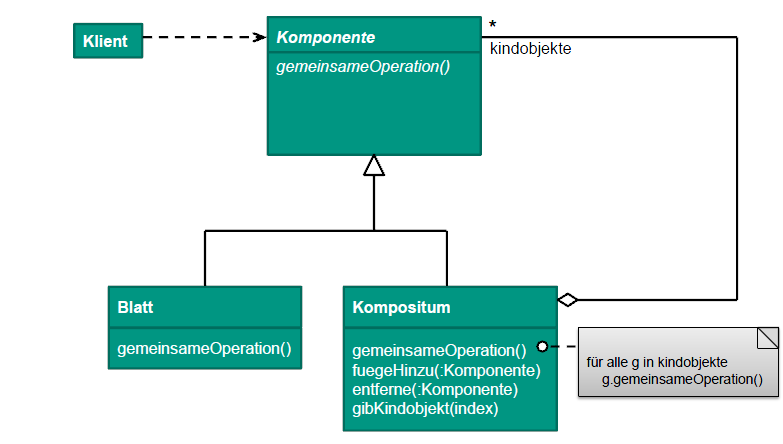
\includegraphics[scale=0.45]{pics/04/KompositumStruktur.png}
	\end{center}

}


\frame {
\frametitle{Zurück zur Aufgabe}
	\begin{block} {Aufgabe (5P)}
Ein binärer arithmetischer Ausdruck enthält einen Operanden, einen Operator (+ - * /) und einen anderen Operanden. Die Operanden können entweder eine Zahl sein oder selbst wieder ein anderer binärer arithmetischer Ausdruck. Entwerfen Sie mit Hilfe eines Entwurfsmusters ein Klassendiagramm, um die Bestandteile eines binären arithmetischen Ausdrucks zu einer Baumstruktur zusammenzufügen und seine Bestands-Hierarchien zu repräsentieren. Nennen Sie das verwendete Entwurfsmuster. Hinweis: z.B. 2 + 3 und (2 + 3) + (4 * 6) sind beide gültige arithmetische Ausdrücke. 
	\end{block} 
}

\frame {
\frametitle {Musterlösung}
	\begin{center}
		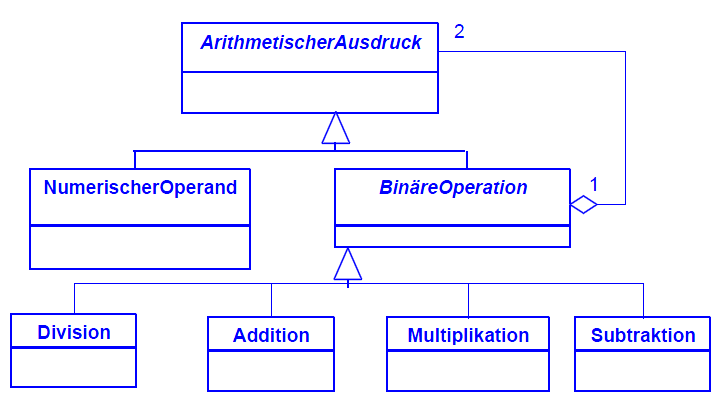
\includegraphics[scale=0.6]{pics/04/KompositumM.png}
	\end{center}
}

\frame {
\frametitle {Beobachter}
\begin{block} {Zweck}
Definiert eine 1-zu-n Abhängigkeit zwischen Objekten, so dass die Änderung eines Zustandes eines Objektes dazu führt, dass alle abhängigen Objekte benachrichtigt und automatisch aktualisiert werden.
\end{block}
\begin{center}
		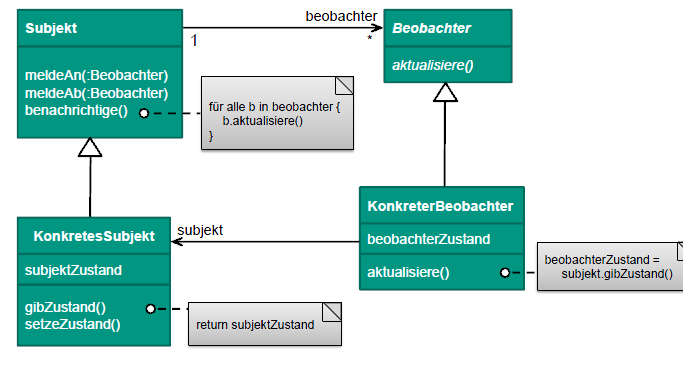
\includegraphics[scale=0.5]{pics/04/beobachter.png}
	\end{center}
}

\frame {
\frametitle {Brücke}
\begin{block} {Zweck}
Entkopple eine Abstraktion von ihrer Implementierung, so dass beide unabhängig voneinander variiert werden können.
\end{block}
	\begin{center}
		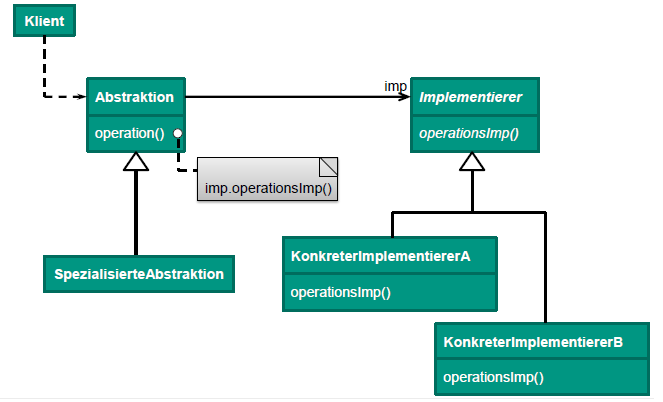
\includegraphics[scale=0.5]{pics/04/Bruecke.png}
	\end{center}
}

\frame {
\frametitle {Aufgabe: Brücke und Beobachter}

Der Begriff Shading bezeichnet in der 3D-Computergrafik im allgemeinen Sinne die Simulation der Oberfläche eines Objekts. Für die Berechnung der Oberfläche gibt es viele verschiedene Verfahren – unter anderem das Flat Shading und das Gouraud Shading. \\
\begin{wrapfigure}{r}{4cm}
	\centering
	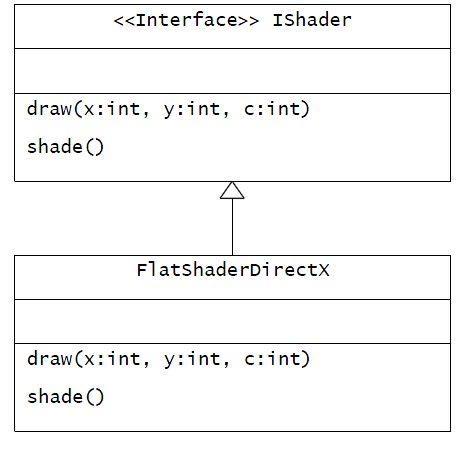
\includegraphics[scale=0.35]{pics/04/BrueckeA.png}
\end{wrapfigure}
Sie haben einen Flat Shader für die DirectX-Programmierschnittstelle entsprechend dem folgenden UML-Klassendiagramm entworfen.
Die Methode shade() in der Klasse FlatShaderDirectX implementiert den Flat Shading-Algorithmus und verwendet die Methode draw(x:int, y:int, c:int), um einen Punkt unter Verwendung der DirectX-Programmierschnittstelle zu zeichnen

}

\frame {
\frametitle {Aufgabe 1 (7P)}
Verwenden Sie das Entwurfsmuster Brücke um die Abstraktion (Methode shade) von der Implementierung (Methode draw) zu trennen. \\
Hinweis: Trennen Sie die obige Schnittstelle IShader geeignet auf und erweitern Sie Ihr UML-Klassendiagramm um die konkreten Klassen DirectXImpl und OpenGLImpl, FlatShader und GouraudShader. Tragen Sie Vererbungsbeziehungen und Assoziationen entsprechend dem Entwurfsmuster Brücke ein. 
\begin{center}
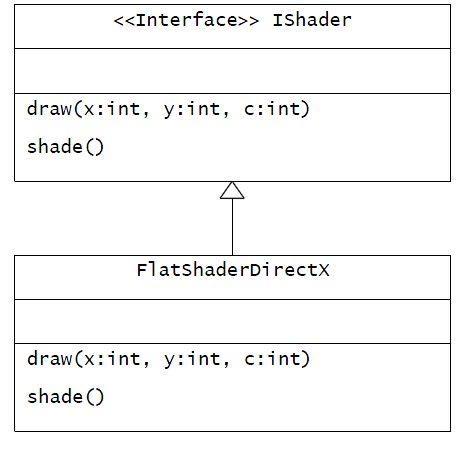
\includegraphics[scale=0.35]{pics/04/BrueckeA.png}
\end{center}
}


\frame {
\frametitle {Musterlösung  (7P)}
\begin{center}
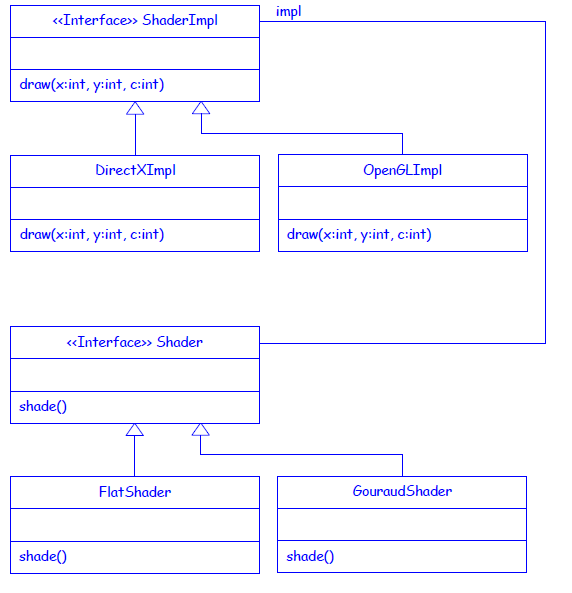
\includegraphics[scale=0.45]{pics/04/BrueckeM.png}
\end{center}
}

\frame {
\frametitle {Aufgabe 1 b(3P)}
\small{Das Gittermodell, für das Ihre Shader-Klassen die Darstellungen der Oberflächen berechnen, wird von der Klasse Gittermodell verwaltet. Bei jeder Änderung des Git-termodells (Subjekt) soll der verwendete Shader (Beobachter) benachrichtigt werden. Verwenden Sie das Entwurfsmuster Beobachter und erweitern Sie das folgende UML-Klassendiagramm um Methoden-Signaturen für das An- und Abmelden, Benachrichtigen und Aktualisieren des Beobachters. \\
Hinweis: Definieren Sie keine zusätzlichen abstrakten Subjekt- und Beobachterklassen sondern verwenden und erweitern Sie lediglich die gegebene Schnittstelle Shader und die Klasse Gittermodell. 
}
\begin{center}
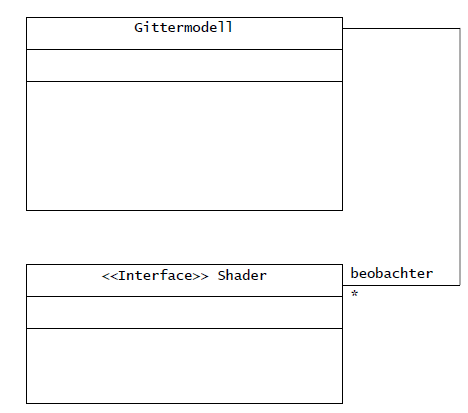
\includegraphics[scale=0.3]{pics/04/BeobachterA.png}
\end{center}
}


\frame {
\frametitle {Musterlösung}
\begin{center}
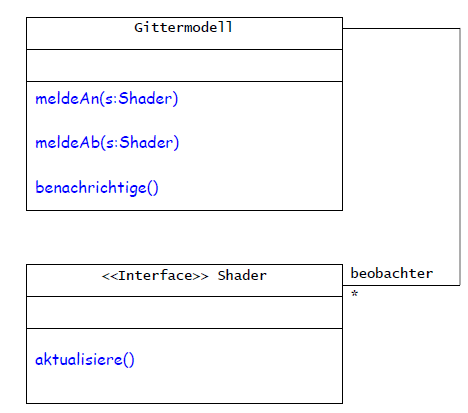
\includegraphics[scale=0.6]{pics/04/BeobachterM.png}
\end{center}
}
\section{Ende}
\subsection{Tipps zum nächsten Übungsblatt}

\frame{
\frametitle{Tipps zum nächsten Übungsblatt}

	\begin{block}{Aufgabe 1 - Entwurfsmuster in der Java-API}
	\begin{itemize}
	\item Falls ihr nicht wisst, was die jeweiligen Code-Stellen tun, "googelt" euch Anwendungsbeispiele
	\item Stellt wirklich nur das allernotwendigste mit UML dar, denn diese Klassen sind recht groß
	\end{itemize}
	\end{block}

	\begin{block}{Aufgabe 2 - Kreuzworträtsel}
	\begin{itemize} \pause
	\item das sollte jeder mit den Entwurfsmustern aus der Vorlesung hinbekommen
	\item achtet darauf, den jeweiligen Namen aus der Vorlesung zu benutzen!
	\end{itemize}
	\end{block}
}


\frame{
\frametitle{Tipps zum nächsten Übungsblatt}
	\begin{block}{Aufgabe 3 - Entwurfsmuster anwenden}
	\begin{itemize}
	\item in beiden Projekten soll genau ein passendes Entwurfsmuster umgesetzt werden, um das Programm einfacher bzw. einfacher erweiterbar zu machen
	\item Abgabe besteht jeweils aus zwei Teilen:

		\begin{itemize}
		\item je ein Klassendiagramm auf Papier
		\item je ein Zip-Archiv mit dem umgebauten Programmcode
		\end{itemize}

	\end{itemize}
	\end{block}
}


\frame{
\frametitle{Bis zum nächsten Mal}
	\begin{center}
	
\includegraphics[height=200pt]{pics/04/04_comic}
	\end{center}
}

\end{document}
